\documentclass[../../main.tex]{subfiles}
\begin{document}

{\bf [解答]}

\begin{figure}[htb]
  \centering
  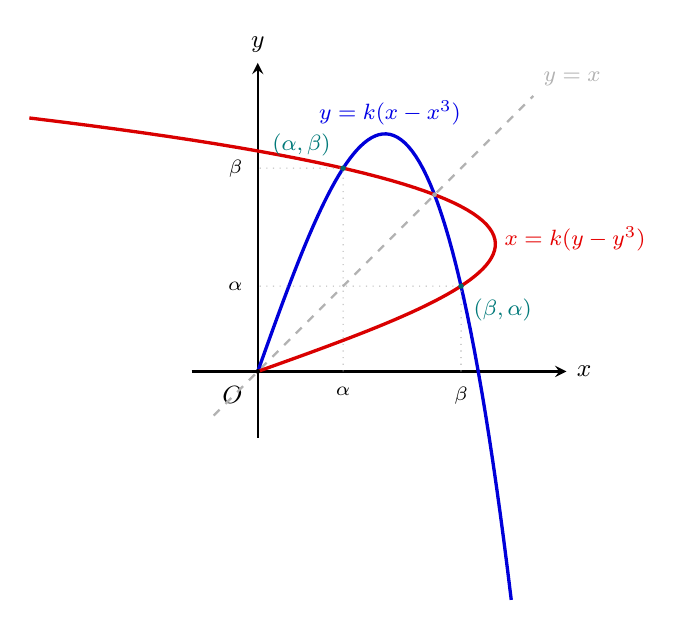
\begin{tikzpicture}[scale=2.8, >=stealth, every node/.style={font=\small}]

    % --- 1. パラメータ設定 ---
    % 例として k = 2.8 (> 2)
    % 1 = alpha^2 + beta^2 かつ alpha*beta = 1/k ≈ 0.357
    % alpha ≈ 0.428, beta ≈ 0.835
    \pgfmathsetmacro{\kval}{2.8}
    \pgfmathsetmacro{\alphaVal}{0.387}
    \pgfmathsetmacro{\betaVal}{0.922}

    \coordinate (O) at (0, 0);
    \coordinate (P1) at (\alphaVal, \betaVal); % (alpha, beta)
    \coordinate (P2) at (\betaVal, \alphaVal); % (beta, alpha)

    % --- 2. 座標軸 ---
    \draw[->, thick] (-0.3, 0) -- (1.4, 0) node[right] {$x$};
    \draw[->, thick] (0, -0.3) -- (0, 1.4) node[above] {$y$};
    \node[below left=2pt] at (O) {$O$};

    % --- 3. 対称軸 y = x ---
    \draw[dashed, gray!60, thick] (-0.2, -0.2) -- (1.25, 1.25) node[above right, font=\footnotesize] {$y = x$};

    % --- 4. 曲線 l_1: y = k(x - x^3) ---
    \draw[very thick, blue!85!black, domain=0:1.15, samples=70]
    plot (\x, {\kval*(\x - \x*\x*\x)});
    \node[blue!90!black, font=\footnotesize, above=10pt] at (0.6, 0.95) {$y = k(x-x^3)$};

    % --- 5. 曲線 l_2: x = k(y - y^3) (媒介変数表示: x = k(t-t^3), y = t) ---
    \draw[very thick, red!85!black, domain=0:1.15, samples=70]
    plot ({\kval*(\x - \x*\x*\x)}, \x);
    \node[red!90!black, font=\footnotesize, right=10pt] at (0.95, 0.6) {$x = k(y-y^3)$};

    % --- 6. 交点 (alpha, beta) と (beta, alpha) ---
    % 座標投影破線
    \draw[dotted, gray!60] (\alphaVal, 0) -- (P1) -- (0, \betaVal);
    \draw[dotted, gray!60] (\betaVal, 0) -- (P2) -- (0, \alphaVal);

    \node[below=2pt, font=\scriptsize] at (\alphaVal, 0) {$\alpha$};
    \node[below=2pt, font=\scriptsize] at (\betaVal, 0) {$\beta$};
    \node[left=2pt, font=\scriptsize] at (0, \alphaVal) {$\alpha$};
    \node[left=2pt, font=\scriptsize] at (0, \betaVal) {$\beta$};

    % 交点のプロット
    \node[circle, fill=teal!85!black, inner sep=0.7pt] at (P1) {}; \node[above left=1pt, teal!95!black, font=\footnotesize] at (P1) {$(\alpha, \beta)$};
    \node[circle, fill=teal!85!black, inner sep=0.7pt] at (P2) {}; \node[below right=1pt, teal!95!black, font=\footnotesize] at (P2) {$(\beta, \alpha)$};

    % y=x 上の交点 (原点および正の交点)
    \node[circle, fill, inner sep=0.6pt] at (O) {};
    \pgfmathsetmacro{\xDiag}{sqrt(1.0 - 1.0/\kval)}
    \node[circle, fill=gray!70, inner sep=0.6pt] at (\xDiag, \xDiag) {};

  \end{tikzpicture}
  \caption{2曲線 $\ell_1, \ell_2$ の概形と $y=x$ 上にない交点 $(\alpha, \beta), (\beta, \alpha)$}
  \label{fig:curves_l1_l2}
\end{figure}

与えられた$2$曲線を
\begin{align}
  \begin{cases}
    \ell_1: y = k(x-x^3) \\
    \ell_2: x = k(y-y^3)
  \end{cases} \label{eq:1}
\end{align}
とする．\cref{eq:1}を満たすような$(\alpha,\beta)$の組が存在するような$k$について考えれば良い．ただし
\begin{align}
  \alpha,\beta > 0, \quad \alpha \neq \beta \label{eq:2}
\end{align}
である．

\cref{eq:1}に$(\alpha,\beta)$を代入して辺々足し引きして
\begin{align}
  \begin{cases}
    \alpha+\beta=k\left\{(\alpha+\beta)-(\alpha^3+\beta^3)\right\} \\
    \beta-\alpha=k\left\{(\alpha-\beta)-(\alpha^3-\beta^3)\right\}
  \end{cases}
\end{align}
である．\cref{eq:2}より$\alpha+\beta \neq 0, \alpha-\beta \neq 0$で両辺を割って
\begin{align}
  \begin{cases}
    1=k\left\{1-(\alpha^2-\alpha\beta+\beta^2)\right\} \\
    -1=k\left\{1-(\alpha^2+\alpha\beta+\beta^2)\right\}
  \end{cases}
\end{align}
を得る．さらに辺々足し引きして
\begin{align}
  \begin{cases}
    0=2k\left\{1-(\alpha^2+\beta^2)\right\} \\
    1=k\alpha\beta
  \end{cases}
\end{align}
で，題意より$k > 0$だから
\begin{align}
  \begin{cases}
    1 = \alpha^2+\beta^2 \\
    \dfrac{1}{k}=\alpha\beta
  \end{cases} \label{eq:3}
\end{align}
である．

\cref{eq:2,eq:3}なる$(\alpha,\beta)$の存在条件を求めれば良い．
$\alpha\beta$平面にこれらを描画すると下図のようになる．

\begin{figure}[htb]
  \centering
  \begin{tikzpicture}[scale=3.2, >=stealth, every node/.style={font=\small}]

    % --- 1. 定数・主要座標 ---
    \coordinate (O) at (0, 0);

    % 円と直線 beta = alpha の交点: (1/sqrt(2), 1/sqrt(2)) ≈ (0.707, 0.707)
    \pgfmathsetmacro{\invSqrtTwo}{1.0 / sqrt(2.0)}
    \coordinate (P_diag) at (\invSqrtTwo, \invSqrtTwo);

    % 例: 1/k = 0.35 (< 0.5) のときの交点
    \pgfmathsetmacro{\cVal}{0.35}
    \pgfmathsetmacro{\alphaPt}{sqrt(0.5 - sqrt(0.25 - \cVal*\cVal))}
    \pgfmathsetmacro{\betaPt}{sqrt(0.5 + sqrt(0.25 - \cVal*\cVal))}
    \coordinate (P_int1) at (\alphaPt, \betaPt);
    \coordinate (P_int2) at (\betaPt, \alphaPt);

    % --- 2. 座標軸 ---
    \draw[->, thick] (-0.15, 0) -- (1.35, 0) node[right] {$\alpha$};
    \draw[->, thick] (0, -0.15) -- (0, 1.35) node[above] {$\beta$};
    \node[below left=2pt] at (O) {$O$};

    % 軸上の目盛り (単位円半径 1)
    \node[below=2pt, font=\scriptsize] at (1, 0) {$1$};
    \node[below=2pt, font=\scriptsize] at ({1/sqrt(2)}, 0) {$\frac{1}{\sqrt{2}}$};
    \node[left=2pt, font=\scriptsize] at (0, 1) {$1$};
    \node[left=2pt, font=\scriptsize] at (0, {1/sqrt(2)}) {$\frac{1}{\sqrt{2}}$};
    \node[circle, fill, inner sep=0.5pt] at (1, 0) {};
    \node[circle, fill, inner sep=0.5pt] at (0, 1) {};

    % --- 3. 除外線 beta = alpha ---
    \draw[dashed, gray!60, thick] (0, 0) -- (1.1, 1.1) node[above right, font=\footnotesize] {$\beta = \alpha$ (除外)};

    % 垂線
    \draw[dashed, black, thick] (0, {1/sqrt(2)}) -- ({1/sqrt(2)},{1/sqrt(2)}) -- ({1/sqrt(2)},0);

    % --- 4. 単位円 alpha^2 + beta^2 = 1 (第1象限) ---
    \draw[very thick, blue!85!black]
    (1, 0) arc[start angle=0, end angle=90, radius=1.0];
    \node[blue!90!black, font=\footnotesize, above right] at (0.75, 0.75) {$\alpha^2+\beta^2=1$};

    % --- 5. 双曲線族 alpha * beta = 1/k ---
    % (i) 接する場合: 1/k = 1/2 (k = 2)
    \draw[thick, gray!70, dashed, domain=0.4:1.15, samples=50]
    plot (\x, {0.5 / \x});
    \node[gray!85!black, font=\scriptsize, right] at (1.15, {0.5/1.15}) {$\alpha\beta = \frac{1}{2}$ ($k=2$, 接する)};

    % (ii) 2点で交わる場合: 1/k < 1/2 (k > 2)
    \draw[very thick, red!85!black, domain=0.28:1.18, samples=50]
    plot (\x, {\cVal / \x});
    \node[red!90!black, font=\footnotesize, right] at (1.18, {\cVal/1.18}) {$\alpha\beta = \frac{1}{k}$ ($k>2$)};

    % --- 6. 交点および除外点のプロット ---
    % 接点 (1/sqrt(2), 1/sqrt(2)) : alpha = beta のため除外（白抜き丸）
    \node[circle, draw, thick, fill=white, gray!80!black, inner sep=0.8pt] at (P_diag) {};

    % 双曲線と円の交点 (alpha, beta), (beta, alpha)
    \node[circle, fill=red!85!black, inner sep=0.7pt] at (P_int1) {}; \node[red!85!black, above right=1pt, font=\scriptsize] at (P_int1) {$(\alpha, \beta)$};
    \node[circle, fill=red!85!black, inner sep=0.7pt] at (P_int2) {}; \node[red!85!black, above right=1pt, font=\scriptsize] at (P_int2) {$(\beta, \alpha)$};

  \end{tikzpicture}
  \caption{$\alpha\beta$ 平面における円 $\alpha^2+\beta^2=1$ と双曲線 $\alpha\beta=\dfrac{1}{k}$ の交点条件}
  \label{fig:alphabeta_plane}
\end{figure}

$k>0$から$0<1/k$にも注意して，従って求めるべき条件は
\begin{align}
  0 < \dfrac{1}{k} < \dfrac{1}{2} \quad \therefore 2 < k
\end{align}
である．$\cdots$(答)

{\bf [別解1]}

最後\cref{eq:3}からの変形だけ何通りか示そう．
まず一つ目は\cref{eq:3}の第一式から$\alpha = \cos\theta, \beta=\sin\theta$とおくことである．
\cref{eq:1}から$0<\theta<\pi/2, \theta\neq \pi/4$である．
これを\cref{eq:3}の第二式に代入して
\begin{align}
  \dfrac{1}{k} = \alpha\beta = \cos\theta\sin\theta = \dfrac{1}{2}\sin 2\theta \quad \left(0<2\theta<\pi, 2\theta \neq \pi/2 \right)
\end{align}
である．この値域を考えて
\begin{align}
  0 < \dfrac{1}{k} < \dfrac{1}{2} \quad \therefore 2 < k
\end{align}
を得る．

{\bf [別解2]}

\cref{eq:3}以下，単に一文字消去しても良い．
第二式より$y = 1/(kx)$だから，\cref{eq:2,eq:3}に代入して
\begin{align}
  &
  \begin{cases}
    1 = x^2 + \dfrac{1}{k^2x^2} \\
    0 < x \\
    x \neq \dfrac{1}{kx}
  \end{cases} \\
  &
  \begin{cases}
    t^2 -t + \dfrac{1}{k^2} = 0 & (t=x^2) \\
    t > 0 \\
    t \neq \dfrac{1}{k}
  \end{cases}
\end{align}
である．故にこれが解を持つ条件を調べる．
$f(t)=t^2 -t + \dfrac{1}{k^2}$とおくと$f(0)=1/k^2>0$および軸が$t=1/2$だから，
$0<t$に$2$解持つことが必要で，条件は判別式が正であること，よって
\begin{align}
  1 - \dfrac{4}{k^2} > 0 \quad \therefore 2 < k
\end{align}
を得る．

{\bf [別解3]}

\cref{eq:3}以下，$\alpha,\beta$を解に持つ二次方程式を考えても良い．
$\alpha$，$\beta$を解とする$2$次方程式を考えてもよい．
$a=\alpha+\beta$，$b=\alpha\beta$とおけば
\begin{align}
  \begin{cases}
    1 = a^2 - 2b
    \dfrac{1}{k} = b
  \end{cases}
\end{align}
だから，考えるべき二次方程式は
\begin{align}
  x^2 - \sqrt{1+\dfrac{2}{k}} x + \dfrac{1}{k} = 0
\end{align}
である．

これが正の異$2$実解を持てばよいので，判別式$D$として
\begin{align}
  D>0 \quad \therefore 1+\dfrac{2}{k} - \dfrac{4}{k} > 0 \quad \therefore 2 < k
\end{align}
である．$\cdots$(答)

\newpage
\end{document}
